%!TEX root = these.tex

%\chapterstar{INTRODUCTION}
% Pour des renseignements sur \chapterstar : voir le fichier macros.tex

\chapterstar{Introduction} % "*" pour que l'introduction ne s'affiche pas dans la table des matières, sinon elle s'y affichera comme un chapitre d
% \mtcaddchapter
% \addstarredpart{Introduction} % Pour ajouter une partie ("part") fictive dans la table des matières
% \mtcaddpart
% \markboth{Introduction}{Introduction}  %% header manuel car sinon, ils me marquent le header du dernier \chapter{?} (on est dans un \chapter*{?} )
\selectlanguage{francais}


\section*{Contexte et problématique}
    La sélection de cibles mobiles est une tâche que l'on retrouve dans de nombreux domaines. Le contrôle du trafic aérien est une application critique, mais relativement aisée du fait, d'une part aux jeux vidéo, en passant par les vidéos interactives (enregistrements d'événements sportifs ou vidéo-surveillance), les simulations scientifiques (mécanique des fluides ou dynamique moléculaire), et les applications militaires. Si la sélection de cibles statiques est un problème bien connu, modélisé par la loi de Fitts et ses nombreuses extensions, et facilité par de nombreuses techniques d'assistance, la sélection de cibles mobiles est plus difficile.
    
	\begin{figure}[h]
		\caption{Écran de contrôle du trafic aérien. Crédit : www.boldmethod.com}
		\centering
		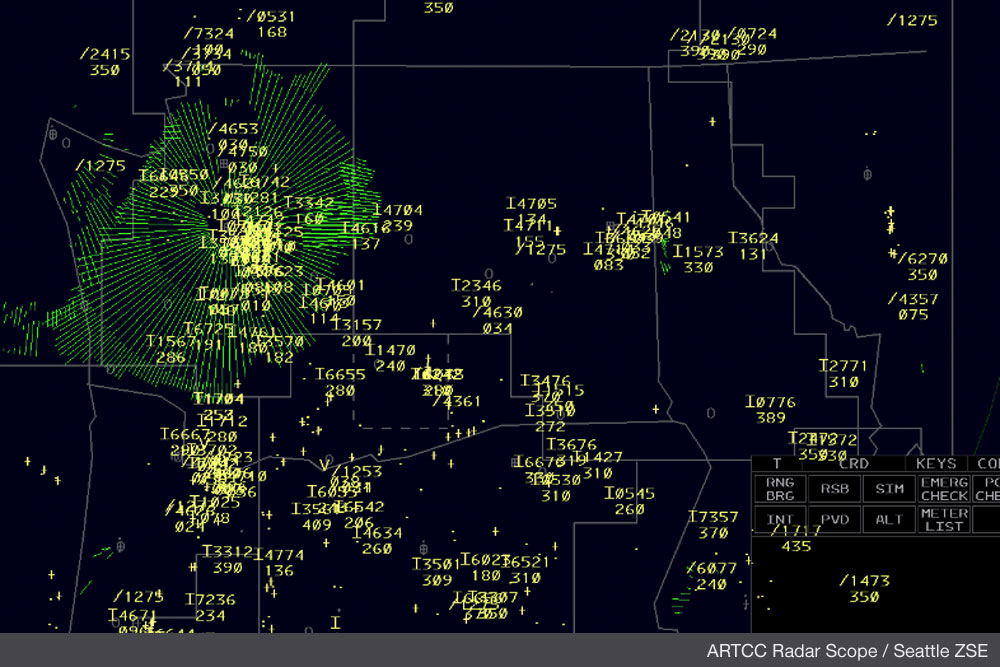
\includegraphics[width=\textwidth]{figures/Radar-Scope-ZSE}
	\end{figure}
    
    Les tendances observées sur les cibles statiques demeurent, à savoir que la difficulté de la tâche augmente quand la distance entre la cible et le pointeur augmente, ou quand la taille de la cible diminue. Mais l'influence du mouvement de la cible empêche d'appliquer la loi de Fitts. Certes, la difficulté de la tâche augmente aussi avec la vitesse, [ref-mec-interact?] cependant, si la nature du mouvement a une importance cruciale, celle-ci demeure peu étudiée.
    
    
    
    
 The
difficulty of the selection increases while (1) target size decreases,
(2) target velocity increases and (3) target density increases. The
selection is even more difficult in 3D environments (filmed or synthetic
environments) because a target of interest can be occluded
by others targets. Selecting someone in crowds with a surveillance
video system is an example of a dense environment with small targets
and occlusion. In some cases, like in action sport footage, both
the objects of interest and the camera can move. Target movements
become unpredictable, and the selection is even more difficult.
In this context, as Hasan et al. [3] wrote, for completing the
selection ”the user must continually track the target and simultaneously
plan to move the cursor over it”. This underscores the key
point of the technique we propose here. Since the user follows the
target for selecting it, the Hook technique tracks the cursor behavior
for assisting the selection. Indeed, observing the history of cursor
displacements, and the history of distances between each target and
the cursor, the system can estimate which target is tracked, and then
propose a selection to the user who just has to validate it. In other
words, the user follows the target of interest, and the system will
know which target it is.
This paper presents the implementation of this technique, and
two experiments which investigate its performance. Hook has been
compared to the basic pointing (non assisted pointing), and to Bubble
cursor [2, 8], for the case of 3D object selection. The first evaluation
involves a desktop configuration, in which pointing is done
on a standard screen with a mouse. The second evaluation involves
an immersive configuration in which pointing is done with a 3dof
(degrees-of-freedom) device. Both evaluations highlight the bene-
fits of this new interaction technique for selecting moving targets in
a 3D environment. More than simply improving the pointing time,
Hook drastically decreases the error rate and allows pointing targets
in high density environments, with high velocity targets that are not
possible to capture with other techniques.


 
\section*{Approche générale}


\section*{Plan du manuscrit}
